\section{Grundlagen}
Im den folgenden Abschnitten werden die benötigten Grundlagen gelegt, um die
im Projekt verwendeten Techniken und Algorithmen zu verstehen. An dieser Stelle
ist anzumerken, dass für detaliertes Verständnis ein Lehrbuch
wie zum Beispiel \cite{hands_on_machine_learning} studiert werden sollte.

Die verwendeten Techniken und Algorithmen werden in den Bereich \emph{Machine
Learning} eingeordnet und umfassen \emph{Neuronale Netzwerke}, \emph{Convolutional Netzwerke},
\emph{Autoencoder} und \emph{Random Forests}. All diese Techniken sind
\emph{supervised} Algorithmen also überwachte Lerner. Damit ist gemeint, dass
den Algorithmen neben den Daten auch die passende Wahrheit in Form von Labels
mit übergegeben bekommen \cite[S. 8]{hands_on_machine_learning}. Dies ist für die
Problemstellung der Hunderassenbestimmung nicht unüblich, da es hierbei um ein
klassiches Klassifizierungsproblem handelt \cite[S. 8]{hands_on_machine_learning}.

\subsection{Neuronale Netzwerke}
Die Entwicklung von künstliche neuronalen Netzwerke (NN) wurden inspiert von den
leistungsstarken biologischen neuronale Netzwerken die in ihrer Gesamtheit
das Gehirn vieler Lebewesen bilden \cite[S. 253-256]{hands_on_machine_learning}.
Zum jetzigen Zeitpunkt generalisieren NN jedoch noch nicht in der Weise
wie es ihre biologische Vorbilder tun. Damit
ist gemeint, dass viele Algorithmen nur spezifische Probleme, die sie gelernt haben,
lösen könen und bisher kaum Transferleistung erbringen können \cite{transferleistung_netzwerke}.

\subsection{Datensatz}
Wie oben angesprochen benötigen überwachte Lernern während des Traningprozesses
die Labels welche die Wahrheit über die Daten enthalten. In disem Fall wäre die
benötigte Wahrheit der Name der Hunderasse. Dementsprechen wird ein Datensatz
benötigt, der die Labels mit enthält. Selbstverständlich könnte ein Datensatz
selber erstellt und gelabelt werden, dies ist jedoch mit einer hohen Arbeitsaufwand
verknüpft. Zusätzlich enthält der Datensatz für jedes Bild Koordinaten
für einen Rahmen (Bounding Box) der den Hund enthält.

Vorteilhafterweise bietet die Internetseite \emph{kaggle} einen gelabelten
Datensatz \cite{datensatz}. Durch diesen wird maximale Anzahl von $120$
Hunderassen die klassifiziert werden soll festgelegt. Insgesamt enthält der
Datensatz $20580$ Bilder die auf die $120$ Rassen aufgeteilt ist. Wie in der
Abbildung \ref{fig:gleichverteilung_bilder} zu erkennen ist, sind die Bilder
gleichmäßig auf die einzelnen Klassen aufgeteilt.
\begin{figure}
\centering
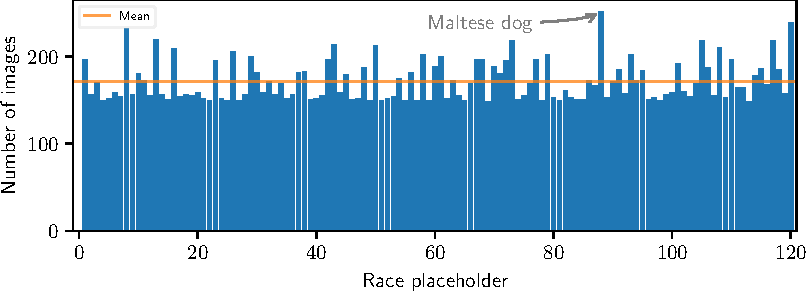
\includegraphics[width=\the\textwidth]{../../final_data/general/image_distribution.pdf}
\caption{Bildverteilung der einzelnen Klassen. Die Namen der jeweiligen Rassen
         wurden durch Platzhalter ersetzt, weil lediglich verdeutlich werden soll
         das die Bilder gleichverteilt sind.}
\label{fig:gleichverteilung_bilder}
\end{figure}
Eine zufällig Auswahl von Bildern des Datensatzes sind in der Abbildung \ref{fig:bilder_cluser}
dargestellt.
\begin{figure}
\centering
\includegraphics[width=\the\textwidth]{../../final_data/general/image_cluster.pdf}
\caption{Zufällig ausgewählte Bilder des Datensatzes.}
\label{fig:bilder_cluser}
\end{figure}
Es ist deutlich zuerkennen, dass einzelne Bilder schwieriger zu klassifizieren sind,
da Menschen, Hindernisse oder andere Hunde im Bild enthalten sind. Außerdem
fältt auf, dass die Auflösung der Bilder nicht homogen ist.

Ein Teil der NN werden auch auf einem kleineren Datensatz mit lediglich $5$ Hunderassen
getestet, um Verarbeitungszeiten zu reduzieren. Dies ist insbesondere bei
der Hyperparamteroptimierung von \textsc{MiniDogNN} wichtig.

\subsubsection{Verarbeitung der Daten}
Um den Datensatz für das tranieren der verschiedenen Algorithmen zu verwenden,
muss er zunächst in einen Tranings-, Validierungs- und Testdatensatz aufgeteilt
werden. Die gewählten Anteile sind $0.6-0.2-0.2$ verwendet und entspricht damit
den in der Literatur \cite[S. 29]{hands_on_machine_learning} empfohlenen Werten.

Während der Tranignsphase werden die Bilder batch-weise geladen und vorprozessiert.
Der Grund für das batch-weise laden ist, dass damit verhindert wird das $20580$
aufeinmal in den Arbeitspeicher geladen werden, was die Leistung der späteren
Traningsphase auf Grund von mangelden Ressourcen beeinträchtigen kann. Die erstellte
Datenlader (Dataloader) Klasse basiert auf der \textsc{keras.utils.Sequence} Klasse die eine
automatische Parallesierung des Ladeprozesses und der Vorverarbeitung ermöglicht
\cite{keras_sequentiel}.

Mit dem Dataloader besitzt die Funktion die Bilder batch-weise auf eine gegebene
Bildgröße runterzuskalieren. Auf die einzelnen Skalierungsgrößen wird in dem
Kapitel \ref{sec:NNarchitekturen} eingegangen, da diese nicht für alle Architekturen
gleich sind. Die batch-weise Reskalierung ist auf Grund der inhomogenität
der Bildauflösungen notwendig, weil \textsc{numpy.array}
eine feste Eingangsform (Input shape) voraussetzen, ergo eine homogene Bildauflösung
innerhalb eines Batches.

Darüber hinaus werden Techniken der \emph{Data Augementation} angewandt, um
die Statistik des Datensatz zuvergrößern. Dies ist sinnvoll, da mit durchschnittlich
$172$ Bildern pro Rassen (vgl. Abbildung \ref{fig:gleichverteilung_bilder})
bei $120$ Rassen, im Vergleich z.\,B. zu Googles \textsc{Open Image} Datensatz
\cite{google_open_image}, wenig Bilder für die Anzahl der Rassen enthält.
Ausdiesem Grund verwenden wir zufällige Rotationen, Translationen und Vergrößerungen
der Bilder, um die allgemeine Statistik zu erhöhen. Hierbei wird sichergestellt
, dass nach einer Translation oder einer Vergrößerung immernoch der ganze Hund
im Bild zu erkennen ist. Hierfür werden die im Datensatz enthaltenten Bounding
Boxes verwendet. Beispielhafte Ergebnisse der Transformationen sind in Abbildung
\ref{fig:data_augementation} dargestellt.
\begin{figure}
\centering
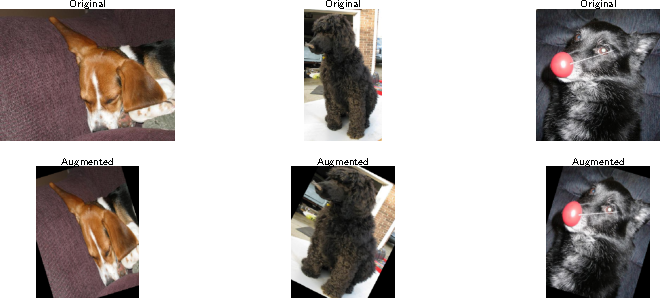
\includegraphics[width=0.8\textwidth]{../../final_data/general/data_augementation.pdf}
\caption{Beispielhafte Transformationen.}
\label{fig:data_augementation}
\end{figure}

\section{Verwendete NN Architekturen}\label{sec:NNarchitekturen}
Der grundsätzliche Aufbau der verwendeten NN ist der Selbe. Um Bilder zu
klassifizerieren müssen informationsreichen Eigenschaften eines Bildes
gefunden werden, sogenannte Features. Hierzu werden NN konstruiert die
Faltungen des Bildes mit einem Filter (Kernel) verwenden. Der Kernel besitzt
Gewichte die tranierbar sind und somit vom Algorthimus optimiert werden können.
Eine solche Netzstruktur wird auch als Convolutional Neuronal Network (CNN)
bezeicht. Die vom CNN generierten Features werden von einem auf Neuronen basierendes
Netzwerk zur Klassifizierung verwende. Diese auch als Fully Connected Network (FCN)
bezeichnete Architekture besitzt als tranierbare Parameter die Matrixelemente
der Neuronenübergangsmatrix. Insbesondere bei FCN ist es wichtig nichtlineare
Aktivierungsfunktion zuverwenden, da ansonsten das Netzwerk nur auf linearen
Abbildung basiert. Das wird bei der Optimierung des Netzwerks zum Problem, da
hier Ableitungen zum Einsatz kommen.

Abgesehen von der Ausgangslage (Output layer) wird Aktivierungsfunktion
\textsc{PReLU} für die CNN und FCN verwendet.
\begin{equation}
  \label{eq:PReLU}
  \map{PReLU}(x)= \begin{cases} x,      & x \ge 0\\
                                \alpha, & \mathrm{sonst}
                  \end{cases}
\end{equation}
Dabei zeichnet sich \textsc{PReLU} dadurch aus, dass der Parameter $\alpha$ in
Gleichung \eqref{eq:PReLU} auch tranierbar ist. Wie in dem Paper (Paper) \cite{he_normal_PReLU}
dargestellt, ermöglicht dies eine schnelleres konvergieren eines Netzwerkes
bei gleichbleibender Wahrscheinlichkeit überzutranieren (Overtraning).
Die \textsc{PReLU} Aktivierungsfunktion ist bereits in \textsc{keras}
implementiert \cite{keras_prelu}. Als Aktivierugnsfunktion für die Ausgnagslage
des FCN wird die bekannte \textsc{sotmax}-Funktion verwendet.Der Ausgabewert dieser
Funktion kann auf Grund der verwendeten Normierung, als Wahrscheinlichkeitsmaß
für die Zugehörigkeit zu jeweiligen Klassen interpretiert werden \cite[S. 139]{hands_on_machine_learning}.
Darüberhinaus wurde auch die Gewichtsinitalisierung für die Kernel und
die Übergangsmatritzen der CNN und FCN angepasst. Hierfür wurde die
bereits in \textsc{keras} implementierte \textsc{he\_normal} Methode
verwendet \cite{keras_he_normal}. Die Vorteile dieser gezielten
Gewichtisintalisierung werden ebenfalls im Paper \cite{he_normal_PReLU} motiviert.

Allgemein ist es möglich bei der Verwendung von CNN eine variable Bildgröße
zu verwenden. Hierdurch kann der maximale Informationsgehalt eines Bildes
verwendet werden. Jedoch wird für FCN eine statische Eingangsgröße benötigt,
um dies zuereichen wird vor der Eingangslage des FCN eine \textsc{GlobalMaxPooling}
Lage (vgl. \textsc{keras} Dokumentation \cite{keras_max_pooling}) verwendet.
Diese verwenden jediglich das Maximum von einem Filter einer Convolutional Lage,
durch die vorab definierte Anzahl an Filtern ist somit auch die Inputgröße eines
FCN festgelegt.
Eine beispielhafte Darstellung über die verwendeten Netzwerkachitekturen findet sich
in Abbildung \ref{fig:beispielhafte_netz_architecture}.

 \subsubsection{MiniDogNN}
 Die \textsc{MiniDogNN}-Architektur ist eine einfach gehaltenes Netzwerk, welches
 in Abbildung \ref{fig:MiniNN} schmeatisch dargestellt ist. In der Abbildung sind
 die Aktivierungsfunktionen nicht mit eingezeichnet. Die Anzahl der Neuronen
 hängt von der Anzahl der Hunderassen $N\ua{dr}$ ab, die klassifiziert werden sollen.
 Darüberhinaus hängt die Anzahl der tranierbaren Parameter $n\ua{train}$ auch davon ab, ob \textsc{RGB} oder
 Graustufen Bilder verwendet werden sollen:
 \begin{align}
   \begin{aligned}
     \label{eq: ntrain_MiniDogNN}
   n\ua{train}\left(N\ua{dr}=5, \,\, \mathrm{grau}\right) &= 21411, & n\ua{train}\left(N\ua{dr}=120, \,\, \mathrm{grau}\right) & = 58096 \\
   n\ua{train}\left(N\ua{dr}=5, \,\, \mathrm{rgb}\right) &= 21555, & n\ua{train}\left(N\ua{dr}=120, \,\, \mathrm{rgb}\right) & = 58240
   \end{aligned}
 \end{align}
 Zwar ist Variabelenenraum gegeben durch die Bildgröße und nicht durch das Bild, wie
 bei einem FCN, jedoch wird in den Gleichungen \eqref{eq:ntrain_MiniDogNN} deutlich,
 dass es deutlich das eine Regularisierung notwendig. Eine Regularisierung
 erfolgt bei der \textsc{MiniDogNN}-Architektur mit Hilfe eine $l2$-Architektur.
 \begin{figure}
 \centering
 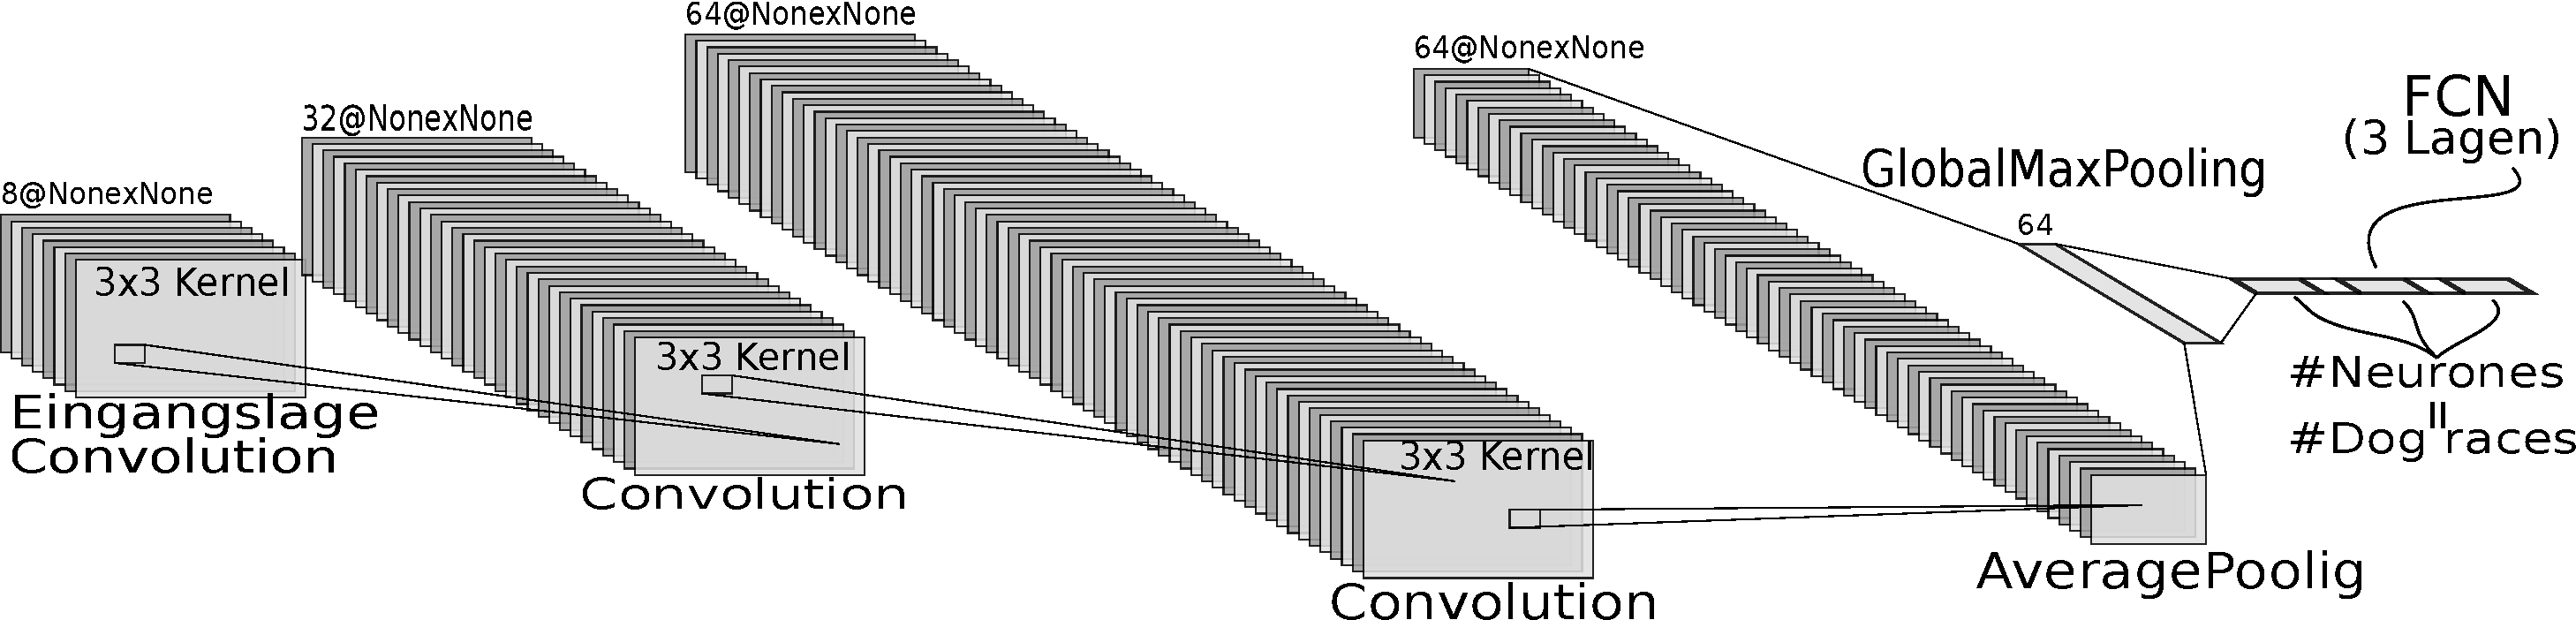
\includegraphics[width=\the\textwidth]{../../final_data/general/MiniDogNN.pdf}
 \caption{Schmatische Darstellung der \textsc{MiniDogNN}-Architektur, wobei
          die Aktivierungsfunktionen nicht mit eingezeichnet sind. Das FCN
          ist schmatisch angedeutet. Erläuterung der Konvention: \emph{\textbf{\#}Filter\textbf{@}Bildbreite \textbf{X} Bildhöhe}.
          Die Grafik wurde unter zuhilfe nahme der Internetseite \cite{net_svg_source} erstellt.}
 \label{fig:MiniDogNN}
 \end{figure}

\subsubsection{PreDogNN \& PreBigDogNN}
Wie im obigen Kapitel angesprochen, ist die Hauptaufgabe eines CNN die Generierung
von Features aus einem Bild. Jedoch limitiert die Größe des Datensatzes stark
die maximalen Größe der \textsc{MiniDogNN}-Architektur. Diese Limitation
kann durch vortrainierte Modelle umgangen werden. Wichtig ist hierbei, dass
ein Modell verwendet wird, dass auch auf Bildklassifizierung ausgelegt ist.
Die Idee ist, den FCN-Anteil des vortrainierten Modells zu entfernen und lediglich den CNN-Anteil
zur Featuregenerierung zu verwenden. Hierbei werden die Paramter des CNN
festgehalten und sind somit nicht tranierbar. An das vortranierte CNN schließt, dann
ein tranierbares FCN an.

Die Modelle \textsc{PreDogNN \& PreBigDogNN} verwenden das CNN der
\textsc{InceptionResNetV2}-Architektur \cite{InceptionResNetV2}. Das Netzwerk
ist in \textsc{keras} vorimplementiert und kann mittels eines Funktionsparamters
in ein CNN umgewandelt werden \cite{keras_InceptionResNetV2}.

Der Unterschied zwischen \textsc{PreDogNN \& PreBigDogNN} liegt in der Anzahl
an Hunderasssen die klassifiziert werden können -
$N\ua{dr, PreDogNN}=5,\, N\ua{dr, PreBigDogNN}=120$. Die Klassifizierung von $5$ Hunderassen
soll an dieser Stelle lediglich mit der Ersparnis an Analysezeit und -hardware
motiviert werden. Bedingt wird die Anzahl an möglichen Hundereassen druch die
FCN-Architektur der beiden Netzwerk. Beim \textsc{PreDogNN} besteht das FCN aus
drei Lagen mit $30-30-5$ Neuronen, im Gegensatz dazu verwendet das \textsc{PreBigDogNN} deutlich
mehr Neuronen innerhalb seiner drei Lagen: $150-120-120$. Die Reduzierung von
$150$ auf $120$ Neuronen in der zweiten Lage ist mit der an der zu tranierenden Paramtern
erklären: Das CNN der \textsc{InceptionResNetV2}-Architektur generiert
$1536$ Features (\textsc{MiniDogNN} $64$) was zu einer Vielzahl von
tranierbaren Gewichten innheralb des FCN führt:
\begin{align}
  \begin{aligned}
  \label{eq:ntrain_PreDogNN_PreBigDogNN}
  n\ua{train}(\mathrm{rgb}) &= 47255 \quad \mathrm{PreDogNN} \\
  n\ua{train}(\mathrm{rgb}) &= 249545 \quad \mathrm{PreBigDogNN}
\end{aligned}
\end{align}
Aus diesem Grund ist hier Regularisierung entscheidend, hierfür wird neben der
$l2$-Regularisierung zusätzlich noch \emph{Dropout} verwendet.

Die \textsc{keras}-Implementierung von \textsc{InceptionResNetV2} benötigt
eine vordefinierte Bildgröße \cite{keras_InceptionResNetV2}.
Aus diesem Grund werden, alle Bilder auf $244\times 244$ skaliert.
Der komplette Datensatz enthält $1735$ Bilder die hierdurch hochskaliert werden.
Es wird der Einfachheit halber angenommen, dass das hochskalieren nur einen
geringen Einfluss auf die Genauigkeit hat. Würde die minimale
Bildgröße der beiden Datensätze verwendet werden (vgl. Abb \ref{} und. \ref{})
würde sich dies negativ auf die Genauigkeit auswirken.

\subsection{Alternative Methode: Autoencoder \& Randomforest}
Als alternativen Ansatz wird ein \textsc{Randomforest} (RF)
in Verbindung mit einem Autoencoder verwendet.
Die hinterliegende Techniken eines RF werden als bekannt vorrausgesetzt und können
gegebenfalls im Buch \cite[S. 181]{hands_on_machine_learning} nachgelesen werden.
Die Features werden in Form eines Vektors an den RF übergeben,
dieser wird mit einem vorab tranierten Autoencoder generiert.

Der Autoencoder verwendet \textsc{ReLU}-Aktivierungsfunktionen
keine spezielle und keine Gewichtsinitalisierung.
Im Gegensatz zu den bisher vorgestellten NN wird hier
\emph{padding} verwendet. Durch das \emph{padding} bleibt die Bildgröße
bei Konvolutionallagen erhalten.
Eine schematische Darstellung des Autoencoders findet sich in Abbildung \ref{fig:Autoencoder}.
Der Autoencoder basiert somit auf Convolutional-Lagen die in Verbindung mit
\textsc{MaxPooling}-Lagen das Bild herunterskalieren. Anschließend wird
mittels \textsc{Flatten} ein Featurevektor generiert der daraufhin durch
\textsc{Reshape} wieder in eine Matrixform umgewandlert wird. Diese wird dann
in den Decoder gegeben, welcher aus \textsc{UpSampling}-Lagen verbundene
Convolutional-Lagen besteht.
\begin{figure}
\centering
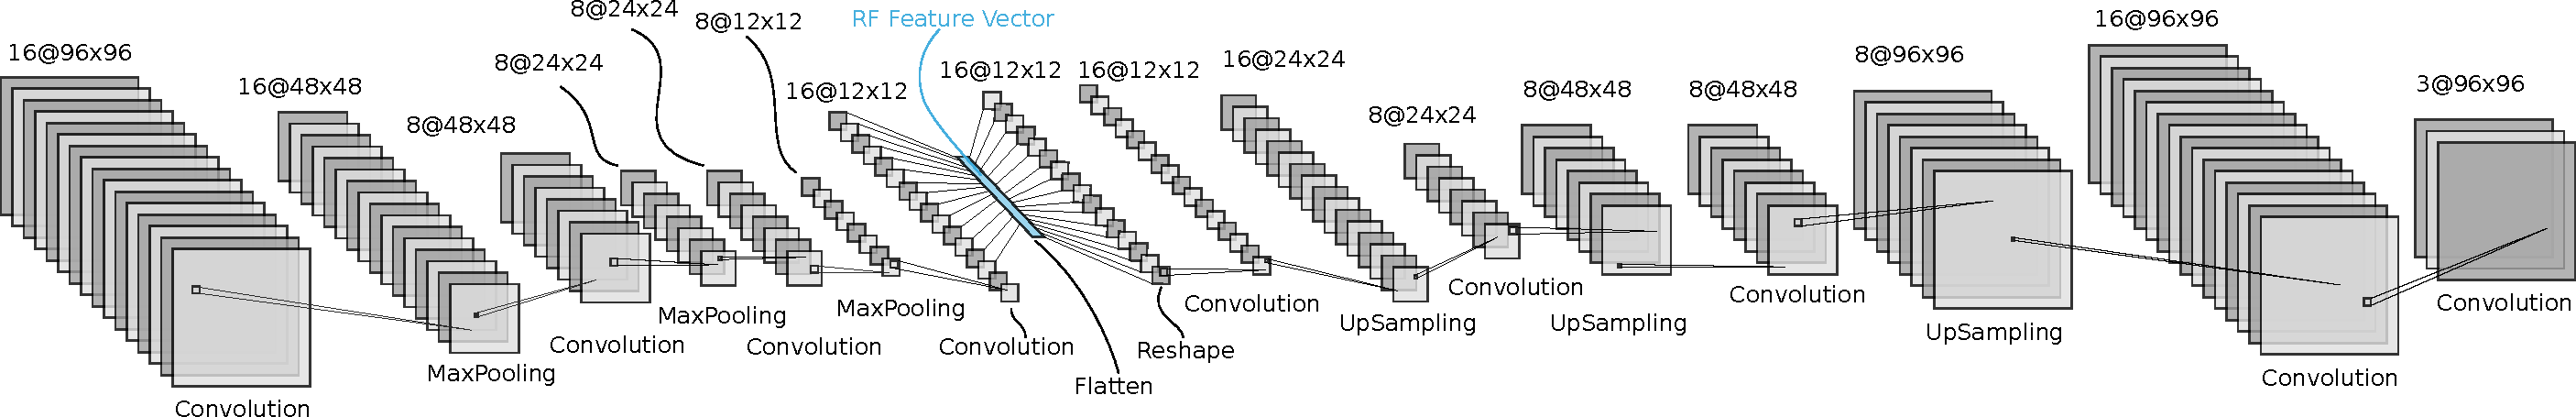
\includegraphics[width=\the\textwidth]{../../final_data/general/autoencoder.pdf}
\caption{Schmatische Darstellung des verwendeten Autoencoders, wobei
         die Aktivierungsfunktionen nicht mit eingezeichnet sind.Das FCN
         ist schmatisch angedeutet. Erläuterung der Konvention: \emph{\textbf{\#}Filter\textbf{@}Bildbreite \textbf{X} Bildhöhe}.
         Die Grafik wurde unter zuhilfe nahme der Internetseite \cite{net_svg_source} erstellt.}
\label{fig:Autoencoder}
\end{figure}
